% This is a sample LaTeX input file.  (Version of 12 August 2004.)
%
% A '%' character causes TeX to ignore all remaining text on the line,
% and is used for comments like this one.

\documentclass{article}      % Specifies the document class


\usepackage{float}							% figure-Umgebung im Text verankern können
\usepackage[pdftex]{graphics}    % Treiber zum Einbinden von Bildern 
\usepackage{graphicx}    
\usepackage{amsmath}
%\usepackage{a4wide}
\usepackage{amsfonts} 

\PassOptionsToPackage{hyphens}{url}\usepackage{hyperref}

\title{FIFO Queue}
\author{ocatias}

\begin{document}             % End of preamble and beginning of text.

\maketitle

\section{Introduction}
In this project we analyze the results of Ruslan Nikolaev's paper  ``A Scalable, Portable, and Memory-Efficient Lock-Free FIFO Queue"\cite{nikolaev2019scalable}. We implement some of his proposed data structures and compare them with two FIFO queues with locks on both operations. Specifically the example 1 and example 2 queues from the lecture.

The main focus of the paper is SCQ (Scalable Circular Queue), a FIFO queue that is ABA safe, livelock free and portable, which is defined as using only widely available single width atomic operations. 

Our goal is to recreate the experiments from \cite{nikolaev2019scalable} and see how the queues compare to queues with locks. Furthermore, we also want to find out whether there are any overlooked cases in which SCQ and SCQP, a queue which builds upon SCQ, perform significantly worse than expected. 

\section{Data Structures}

\subsection{Preliminaries}
The datastructures we are implementing are all First-In First-Out (FIFO) queues. They have two operations: ``enqueue$(x)$'' which takes an element $x$ and saves it in the queue and ``dequeue()'' which returns the oldest value in the queue.
 
SCQ has a constant $n$ which is assumed to be the upper bound on the number of threads simultaneously possible at the same time. For SCQ $n$ needs to be set to a power of 2, i.e. $n = 2^b$ with $b\in \mathbb{N}$.   Furthermore, SCQ is designed in such a way that there is a connection between $n$ and the number of entries that can be saved into the queue (its capacity) and the amount of data that each entry can store: The capacity of the queue has to be $2n$ and the number of bits of data we can save per entry is $b+1$ where $n= 2^b$.  This has the obvious downside that we can only store data of a limited size directly in the queue. Furthermore, the amount of data we can save in an individual entry is correlated to the required capacity of the queue. For example if we want to store a numbers from $0$ to $2^{20}-1$ then the queue needs to be able to store $2^{20}$ entries.


\subsection{The Scalable Circular Queue}
\subsubsection{Overview}
The data of SCQ is stored in a ring buffer of size $2n$. The ring buffer wraps around, i.e. writing to the $(2n+k)$-th index will write to the $k$-th array entry. This allows us to monotonically increase the head and tail pointers, without worrying about them getting too big\footnote{Except of course when they overflow.}. 

The head and tail pointers help us find the oldest entry or the next free one respectively. 
We increment the tail pointer whenever we enqueue an element, and increment the head pointer whenever we dequeue an element.
%They get incremented by one whenever we enqueue or dequeue an element. 
The pointers have the form of $x =j + i \cdot 2n$ where $j$ is the ring buffer index of the element, $i$ the current cycle and $2n$ the ring buffer size. If $x$ is the pointer, we can then get the index by $index(x) = x \textrm{ mod } 2n$ and the cycle by $cycle(x) = \lfloor x / 2n\rfloor$. The cycles count how often we have gone through the entire ring buffer. We can use the cycles to determine when an element was saved into the queue.

At each of these $2n$ indices we can store an entry. For our implementation, these entries are 64 bit unsigned integers. Each entry consist of $b+1$ bits of data (where $n=2^b$ and $b \leq 61 $), a safety bit and $(64 -(b+2))$ bits that store the cycle in which the entry was saved.

We reserve the biggest number $2n -1$ that we can store into the SCQ as a special value we will call $\bot$. Its purpose is to mark an entry as empty.

To \textbf{enqueue} we use FAA to increase the tail pointer by one. It now points to an entry that we have not written to in this cycle. If this entry is from a previous cycle and empty (signaled by $\bot$) we compare and swap (CAS) our data and the current cycle of the tail into to this entry, otherwise we reload the tail pointer and try again.

\textbf{Dequeuing} works similarly: we increase the head pointer using FAA and check whether that entry is from the current cycle (the cycle of the head pointer), if it is we mark it as empty ($\bot$) with an atomic OR operation and return its data. We can use an OR for this because we previously defined $\bot = 2*n -1$ as the biggest number we have enough space to save. Since $n$ is a power of 2 this means that the binary representation of $\bot$ consists only of 1's. So if we use an OR on the entry's data and $\bot$ then the data part of the entry will be completely overwritten by 1's, meaning that it is equivalent to $\bot$.


\subsubsection{Details}
Most of SCQ's complexity comes from making sure that all of the queue properties hold and that it works efficiently. We will now explain the inner workings of SCQ in a bit more detail. To completely understand SCQ it is probably best to take a look at the pseudocode in \cite{nikolaev2019scalable}.

SCQ uses a \textbf{threshold value} to help us determine if the queue is empty: if $threshold < 0$ then we know that the queue is empty. This allows us to not waste time searching for a nonexistent entry if we know that the queue is empty. Whenever a dequeuer\footnote{A dequeuer is a thread that is currently doing a dequeue operation.} reads an entry that it cannot return, the threshold value gets reduced by one. This means that we need to set the threshold value to the number of unsuccessful dequeuer reads after which we can be sure that the entire queue is empty. In \cite{nikolaev2019scalable} it is shown that the threshold value has to be $3n-1$. The threshold gets reset to $3n-1$ whenever an enqueue operation is successful.
%By assumption: $n$ is the upper bound of possible concurrent enqueuers or dequeuers and $2n$ the size of the ringbuffer. This means if there is an entry in the queue it is always at most $2n$ spots away from any dequeuer. In this scenario we can also have up to $n-1$ dequers that potentially fail the dequeue and this reduced the threshold value. This means that we need to set the threshold value to $(N_{max \ dequeuers}) + (N_{queue\ size}) = (n-1) + 2n = 3n -1$  to make sure that a dequeuer can always find the last enqueued element. This is our threshold value, the current threshold gets reduced by one for each time a dequeuer unsuccessfully tries to dequeue an entry and it gets reset to $3n-1$ whenever we enqueue an element.

As mentioned above we reserve a bit in every entry that is called the \textbf{isSafe} bit. We do this to solve the following problem: assume a dequeuer arrives at a non-empty entry where an enqueuer\footnote{An enqueuer is a thread currently doing an enqueue operation.} from a previous cycle wants to write its value. If the entry becomes empty and we let the enqueuer write its value then we will never be able to dequeue this value as a dequeuer can only return values from its own cycle. Since the dequeuer is already at a bigger cycle than the enqueuer and the cycles of the dequeuers cannot decrease we will never have a dequeuer that has the same cycle as the entry. Thus we need to stop the enqueuer from writing to this entry. For this we use the \textbf{isSafe} bit:
whenever a dequeuer arrives at an entry that is occupied (but not yet written to) by an enqueuer from a previous cycle, the isSafe bit is set to false via CAS. Enqueuers make sure to only write to an unsafe entry when the head pointer is not in front of the tail pointer to avoid this problem. The \textbf{isSafe} bit will only be restored to true once a new value is stored at this index.

The final detail we will mention here is the \textbf{catchup procedure}. Whenever a dequeuer detects that the tail is behind the head, it calls \textbf{catchup procedure} which pushes the tail forwards. This is to avoid unnecessary iterations in the enqueue function. 

%We reserve a special value $\bot$, for this we use the biggest possible index $2n-1$\footnote{This is because $n$ is a power of 2.}. This value signals that the corresponding slot is empty and can be written.

%\textbf{Enqueue:} To enqueue we get the index\ref{fn:cache_remap} of an entry from the tail pointer and load the corresponding entry. We make sure to only store data on entries that are marked as free (i.e. they have the entry $\bot$), from previous cycles and, whose isSafe bit is 1 or the Head is not ahead of the tail. We use CAS to store the entry (resetting the isSafe bit to 1) and restore the threshold to $3n-1$. 

%We now go through all of the cases that can happen during a \textbf{dequeue} operation: 
%\begin{itemize}
%	\item $threshold < 0$: Queue is empty return $\bot$
%	\item $cycle(entry) = cycle(head)$: Because head increases monotonically before each read, we know that this is an unread entry. We overwrite its index to $\bot$ with an atomic OR operation and return its index.
%	\item $cycle(entry) < cycle(head) \ \& \& \ index(entry) = \bot$: A dequeuer arrived at this node before an enqueuer, use CAS to increase the cycle of this node to $cycle(head)$ to make it impossible for the enqueuer to store its value there.
%	\item $cycle(entry) < cycle(head) \ \& \& \ index(entry)\neq \bot$: An enqueuer has arrived to the entry before the dequeuer, we use CAS to mark it as unsafe.
%	\item If a CAS fails we reload the current entry and check it again.
%	\item If no  CAS fails or none of the above cases apply:
%	\begin{itemize}
%		\item $Tail \leq Head +1$ the queue is empty, we call catchup and return $\bot$
%		\item $Threshold < 0$ The queue is empty, return $\bot$
%	\end{itemize}
%\end{itemize}

\subsubsection{Further SCQ Optimizations}
\label{sec:scq_optimizations}
The original paper presents two optimizations of SCQ. The first one is that when a dequeuer arrives at an entry before its corresponding enqueuer it spins for a short amount of time before it invalidates the entry. We benchmarked different numbers of spins in section \ref{sec:bench_opt}. This optimization seems to only have a small impact and the different spin numbers all have their up- and downsides. We chose a spin number of $1000$ as it had the best performance when it came to 50\% enqueue operations on an empty queue (more on that in section~\ref{sec:bench_opt}).

Unfortunately, the description of this optimization is not very clear in \cite{nikolaev2019scalable}. After doing all of our experiments we noticed that we most like made a small mistake in the implementation of this feature, which makes a slightly less efficient.\footnote{Instead of only letting the thread spin whenever the dequeuer arrives before the enqueuer our more inefficient implementation also spins when it wants to set the \textbf{isSafe} bit to false.} However, tests showed that these speed differences between implementations were not really consistent\footnote{In some cases the ``improved version'' was faster, in some it was slower. We think this implies that the speed differences are just random fluctuations.} and mostly smaller than the differences observed when rerunning the exact same tests. So I decided not to redo all of the experiments, since I thought that there are many other students who might need to use the Nebula server. The reason I noticed the mistake in our implementation is because of \cite{10.1145/2517327.2442527} which is that paper that inspired the SCQ, so if one wants to learn more about the way SCQ works it might be a good idea to also study \cite{10.1145/2517327.2442527}.

The second optimization is using ``cash remapping" so that neighboring entries lie on different cachelines. Again, the author has not specified how this works and neither could I find more information about this anywhere else. This is why I came up with my own cash remapping function:
\begin{equation}
	f(x) = \frac{2n}{64}(x \ \mathrm{mod} \ 64) + \left\lfloor \frac{x}{64} \right\rfloor
\end{equation}
To understand the results consider the transformation on a queue with capacity 4096: we take as input the indices $(0,1,2,3,...)$. Applying cache remapping to these indices gives us $(0,64,128,192,...)$. As you can see, the function makes sure that neighbors get separated by 63 indices, which makes sure that they are not on the same cacheline. I have not analytically proven that this function is generally correct. However, a bruteforce search found that it yields valid indices for all queue capacities from $2^6$ to $2^{28}$ which should be enough for all current applications.

\subsubsection{A Note on the Implementation of SCQ}
Implementing SCQ was pretty straightforward. For most parts the pseudo code in \cite{nikolaev2019scalable} is clear. There are no detailed instructions on how to implement the different kind of informations stored in the entries (cycle, data and $IsSafe$). However, we managed to do this with the help of a few basic bit operations.

Something that was more of a challenge to us was the implementation of $n= 2^b$. We need to know the value of $b$ for every operation. Storing $b$ as just a normal integer seemed like a bad idea to us as we do not know how this would influence the performance when it comes to multiple threads reading $b$.\footnote{None of the threads change $b$, so intuitively this should not influence the performance, but I am not experienced enough to say this for sure.} We came up with three initial solutions to this problem: hardcode $b$, set $b$ to constant or require that $b$ is given as a parameter for every operation\footnote{After implementing our final solution, we found on Nikolaev's GitHub page that this is how he solved this problem.}. The first two solutions have the downside that you cannot change $b$ without changing the program code, this is obviously bad design and not very flexible. The second option has the downside that if during any operation a false $b$ is given as a parameter then this can lead to various problems. In the end we solved this problem using templates. When using SCQ one now needs to give $b$ as a template parameter for example  \textit{scq$<$16$>$ Q} instantiates SCQ with $b=16$. This has the advantage that template parameters get evaluated by the compiler, meaning that this behaves exactly as if $b$ was hardcoded, but without the downside of $b$ being fixed.

\subsection{SCQP}
\label{sec:SCQP}
SCQP is a variant of SCQ that can store pointers. There are two different variants of this datastructure in the paper that are both called SCQP:

The first one is built with a SCQ that uses double-width CAS, this allows it to directly store pointers. However, as this is not portable and not the focus of the paper, we did not implement it. 

There is a second way of storing pointers (or any kind of data) with the help of a SCQ. Instead of saving the data directly in the queue we store the data in an external array at some index and use SCQ to manage the indices. This gives us another SCQP data structure. 

This variant works the following way: We instantiate an array and two SCQs which we call \textbf{aq} and \textbf{fq}, one collects the indices of entries where we have \textbf{a}llocated data (\textbf{aq}) and one collects the unallocated \textbf{f}ree indices (\textbf{fq}). To enqueue data we dequeue a free index from \textbf{fq}, save the data in the array at this index and put the index into \textbf{aq}. To dequeue  we dequeue an index from \textbf{aq}, collect the data from the array and put the index into \textbf{fq}. This has the advantage that \textbf{aq} and \textbf{fq} do not need to be able to detect when they are full, they only need to detect when they are empty. Which means that SCQP can use the emptyness from one of the SCQs to find out whether it is full or empty. This is because before we can enqueue an index we need to dequeue it from the other queue, therefore if one of the queues is full then the other has to be empty. 

This variant has the downside that any operation (enqueueing or dequeueing) on the SCQP requires both an enqueue and a dequeue operation on SCQ. As such we expect the SCQP to perform significantly worse than SCQ.

\subsection{LSCQ}
The paper also introduces a further data structure called LSCQ, an unbounded SCQ-based queue. We did not implement this data structure, as it is not the focus of the paper and just a small variation of SCQ. Note that Nikolaev also did not implement or benchmark this data structure. 

One thing we noticed about LSCQ: in the pseudocode the author uses double-width CAS SCQ, as it can store pointers directly. For an architecture that does not support double-width CAS one would need to use a SCQP that uses two SCQs, which would probably severely impact the performance. 

\subsection{Properties}
The SCQ is lock-free, linearizable and ABA safe. ABA safety follows directly from way we count cycles. The cycles get incremented monotonically since head and tail also get incremented monotonically and wraparounds only happen after more operation than the CPU word's largest values.  

The author does not directly mention any properties of the SCQP. However, as the SCQP uses basically only SCQ operations (and reading/writing to an array) the only way for it to lock is when SCQ locks, so since SCQ is lock-free so is SCQP.\footnote{There is another way the SCQP could lock: this would happen if we enqueue more indices into one of its SCQs than its capacity. But this is not possible by construction.} Since the result of SCQP is only dependent on the results from SCQ it follows that since SCQ is linearizable, so is SCQP. A similar argument can be made for ABA safety.

Another property of SCQ is that it cannot detect when it is full, i.e.\ a thread that enqueues a value to a full SCQ will spin until it can store its value. Nikolaev mentions a variation that would allow SCQ to detect that at least $n$ elements are in the queue, but this method is supposedly imprecise. SCQP does not have this problem as mentioned in section~\ref{sec:SCQP}.

\section{Evaluation}
We implemented SCQ, SCQP (with 2 SCQs) and the example queues 1 and 2 with locks from the lecture, henceforth referred to as BLQ1 and BLQ2. We also implemented an additional queue from the paper called NCQ\footnote{NCQ is a precursor to SCQ. In the paper it is used to introduce some of the basic concepts necessary for SCQ. As NCQ is not the focus of the paper we also did not make it the focus of this project.}, but we did not extensively test nor benchmark it due to time constraints. We made two small changes to BLQ1. First, we use an array with head and tail pointers instead of a linked list, this is to bring it closer to the implementation of SCQ which also uses an array with head and tail pointers. Second, when our variant detects that it is empty it does not spin and wait for a new element, instead it reports that it is empty. This is the same way SCQ deals with dequeues when empty. If we would allow it to spin while empty this would strongly disadvantage BLQ1 during benchmarking.

\subsection{Testing Basic Queue Functions}
To test if our FIFO queue objects behave according to expectations we implemented several tests. 

The first one creates many threads that perform enqueue-dequeue pairs\footnote{Since this will also be important later on, let me clarify that this means that the operations for a single thread then look like: enqueue(x), dequeue(), enqueue(y), dequeue(), ...} in rapid succession and after each dequeue we check whether the dequeue operation returns an element. While this test seems very simple it actually found the most complicated error in the code: there was a small bug in the code that only was triggered when a dequeuer arrived before its corresponding enqueuer. This bug also only happened when the enqueuer and dequeuer were on different cycles. All of this meant that the bug only happened when the enquque and dequeue operations proceeded at full speed which meant that outputting too much information during these operations lead to the bug not happening. This made it very hard to locate and fix the bug.

The second test creates many threads that all enqueue unique values. Then a single thread dequeues all of the values and we make sure that for each thread no element gets returned before an earlier enqueued element. This means if for some thread $i$ $enq_i (j) \rightarrow enq_i (k)$ (i.e. thread $i$ enqueues $j$ before it enqueues $k$) then it always has to hold that $deq_l(j) \rightarrow deq_m(k)$ for arbitrary threads $l, m$. This tests whether all the elements get returned in their sequential order (relative to their thread). 

The third test creates many threads that randomly either enqueue or dequeue elements. Afterwards we dequeue all of the remaining elements from the queue. We collect all the dequeued and enqueued elements and check whether they are exactly the same without any missing. 

\subsection{Experiment Design}
We decided not to test the basic properties of SCQ and SCQP because they are either very hard to test for (ABA safety) or they follow directly from theory (ABA safety, lock-freedom and linearizability). We identified two interesting metrics to benchmark: throughput and latency. Throughput is defined as the number of operations in some time interval and latency is the average time per operation. If we had a perfect concurrent data structure we would expect its throughput to scale (up to linearly) with the number of threads. Compared to that, the latency of a perfect data structure would probably stay constant with the number of threads. As the paper uses throughput for its experiments we also decided to use throughput. 

This is where we also had the first big problem with the implementation of the benchmark: instead of measuring the time it took for all the threads to finish, we measured the time intervall of each thread separately and then added them up. This meant that instead of measuring the throughput we actually measured $1/\mathrm{latency}$. This obviously produced very unexpected results.

The experimental setup we decided on is the following: we create a new queue $Q$ and then have a fixed number of threads $k$ perform $O$ operations each. We measure the time $t$ it takes to perform all of those $O\cdot k$ operations which gives us the throughput $T = \frac{O\cdot k}{t}$. We repeat this 35 times and report the mean value and the standard deviation. To make sure that all threads perform their operations concurrently, we use a barrier that only lets q thread pass if all of the threads are at the barrier. Additionally we use the barrier to start the time measurement, which makes it more precise. 

An alternative setup would be to have $k$ threads execute as many operations as possible in some time interval $t$ and then use this to calculate the throughput. This has the upside that when one thread pauses then this will only slightly change the results. Contrary to this, if one threads pauses in the first described setup, then we need to wait till it completes to finish the time measurement meaning that this drastically changes the result. However, we decided to use the first setup as it is closer to the setup used in the paper. 

Another interesting alternative could be to create threads that do different things, for example an experiment where each thread performs only enqueue or only dequeue operations. Something that could also be useful is to have $k-1$ threads perform the same operations and have one thread that only dequeues until all other threads have completed their operations. This would mean that the queue could never freeze due to being full and all threads waiting to enqueue a value.\footnote{The reson for this is that even if the queue reaches maximum capacity then the ``only dequeue'' thread will make sure to dequeue entries so that the other threads can continue.} A setup like this would give us way more freedom to choose an operation mix for the other $k-1$ threads.

Given our setup above, there are two more things we can adjust for this experiments: the state of the queue and the mix of operations. When it comes to the mix of operations the paper performed four different kinds experiments: only dequeues, enqueue-dequeue pairs, and enqueues and dequeues with a 50\% probability each. We used all of those operation combination and added two more: enqueues and dequeues with a 99\% probability of dequeuing, and enqueues and dequeues with a 70\% probability of dequeuing. The reasons for these two experiments will be explained in section~\ref{sec:bench}.

\subsubsection{The State of the Queue}
\label{sec:state_of_Q}
There are two primary things we can adjust when it comes to the state of the queue: how much it is filled at the beginning and its capacity. In \cite{nikolaev2019scalable} is simply stated that that the queue was measured in a 'steady/hot-state' and never elaborated what this means. We think this means his queues were already prefilled to a certain percentage but we cannot be sure. We chose to do our experiments both with empty queues and with queues that are 45\% prefilled. This number was determined experimentally as being as big as possible while still being small enough so that our queues do not reach their maximum capacity and freeze.

When it comes to tuning the capacity it becomes complicated. In the paper Nikolaev used a capacity of $2^{16}$ and applied $10^7$ operations to this queue which they repeated 10 times for each data point. However, we need to repeat all of our experiments more than 30 times and we expect some of our queues to be notably slower than SCQ. This means that we cannot do as many operations. Unfortunately, we cannot tune the capacity of the queue and the number of iterations separately as we want to have our queue go through a similar number of cycles as Nikolaev's queue. This is because we want to give the enqueuers and dequeuers the possibility to spread over multiple cycles, which is simply not possible if the test runs for only one or two cycles. From the given number of operations and the capacity we estimate that the tests in the paper ran for  $\frac{10^7}{2^{16}\cdot 2} \approx 76$ cycles. With this in mind we designed our own experiments: $5\cdot 10^5$ operations on a queue with capacity $2^{12}$ repeated 35 times for each data point. This means our experiments will run for approximately $\frac{5\cdot 10^5}{2^{12}\cdot 2} \approx 61$ cycles which we think is close enough to the number of cycles in \cite{nikolaev2019scalable}.


\subsection{Benchmarking Details}
\begin{table}[]
	\begin{tabular}{|l|l|l|l|l|}
		\hline
		Processor Name         & Processor Details      & RAM    & L3 Cache & Hyperthreading \\ \hline
		Intel Xeon E7-8880     & 4x18 cores at 2.30 GHz & 128 GB & 45 MB    & No             \\
		POWER8                 & 8x8 cores at 3.0 GHz   & 64 GB  & 8 MB     & Yes            \\
		AMD EPYC 7551 32-Core & 2x32 Cores at 2.0 GHz  & 256 GiB & 8 MB     & No             \\ \hline
	\end{tabular}
	\label{tab:pcs}
	\caption{The PCs that were used for benchmarking, row one and two (called PowerPC) were used in the original paper and row 3 is the Nebula system which we used.}
\end{table}
 We benchmark BLQ1, BLQ2, SCQ and SCP to compare them with each other. For this we use the Nebula system (see tab. \ref{tab:pcs} row 3). We programmed in C++ with C++ threads. Initially we wanted to use OpenMP for this task, but BLQ1 needs a reentrant lock to work. Since OpenMP does not offer such a lock, we had to switch to C++ threads in the middle of the project. We compiled with gcc 8.3.0 on Debian 4.19.98-1 and the -O3 flag. \\
The paper contains benchmarks of the SCQ and the SCQP on two different computers, which can be seen in tab. \ref{tab:pcs} (row 1 and 2; we will refer to the PC from row 2 as the ``PowerPC'').
 The PowerPC does not support double-width CAS which is why Nikolaev had to use a SCQP variant with 2 SCQs. Since the Intel machine used SCQP with double-width CAS, this makes comparisons between the benchmark results of the SCQP between these two machines very hard. Nikolaev used the following benchmarks: dequeues on an empty queue, memory consumption, enqueue-dequeue pairs, and randomly enqueueing and dequeueing with a 50 \% probability for each.
 
We did replicate all of these benchmarks with exception of the memory consumption one since BLQ1, SCQ and SCP have very similar memory requirements and BLQ2 just grows linearly with the number of elements enqueued. 

These benchmarks left us with two questions: What happens if we do tests in a non hot state i.e. what happens if the queue starts out empty? If we randomly enqueue and dequeue values, what happens if one operation is more likely to happen than the other?\footnote{If $p$ is the probability for an enqueue to happen, then running long tests with $p > 0.5$ is not feasible since SCQ has a maximum queue capacity. This is why we focus our tests on cases where $p \leq 0.5$.} 

%The choice of $n$ also seems rather important. If we increase $n$ we can store more and longer data; increasing it also means that more threads can access the queue at the same time. It would be interesting to see how the queue behaves at different values for $n$. Finally, what happens if we have threads that are dedicated to either only enqueueing or only dequeuing values?


\subsection{A Few Initial Hypotheses}
\label{sec:initial_theories}
Before we start benchmarking we will form some hypotheses about how we expect the queues to behave and then see if the experiments agree with our assumptions.
\begin{itemize}
	\item \textbf{BLQ1 and BLQ2:} both use locks so we do not expect any speedup as the number of threads increase.
	\item \textbf{Empty dequeues:}  When it comes to empty dequeuing both SCQ and SCQP should behave more or less equally: atomically load the threshold value, notice that it is less than 0 and return. Hence, we expect SCQ and SCQP to be very fast in this experiment. We also expect SCQ and SCQP to scale very well with the number of threads.
	\item \textbf{SCQ vs SCQP:} Since SCQP uses two SCQ operations for each enqueue/dequeue operation, we expect it to perform worse than SCQ. The only exceptions is when the queue is empty (see above) or full.
\end{itemize}

\subsection{Benchmarking Results}
We will now present the results of the benchmarks. As previously mentioned all of our experiments were conduced 35 times and we report the average value and the standard deviation.
\label{sec:bench}
\begin{figure}[hbtp]
	\centering
	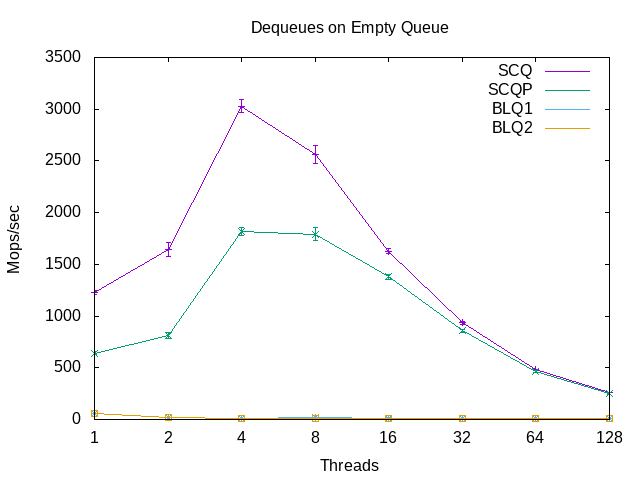
\includegraphics[width=0.75\textwidth]{Pictures/tp_deq_empty.png}
	\caption{Throughput of dequeues on an empty queue}
	\label{fig:tp_empty}
\end{figure}

Fig. \ref{fig:tp_empty} shows the results of doing dequeues on an empty queue. As we can see, both SCQ and SCQP are significantly faster than BLQ1 and BLQ2. The throughput of SCQ and SCQP increases for up to 4 threads and afterwards drops. This is unlike both the paper and our hypothesis: as only an atomic load is necessary we would expect it to scale really well. I spent a lot of time on figuring out why this happens but could not locate a problem in our program. Of course the problem could also be with the CPU as we compare results measured on different CPUs. Benchmarks of inner performance counters (see section~\ref{sec:diss}) also did not give us any explanation for why this happens.

\begin{figure}[hbtp]
	\centering
	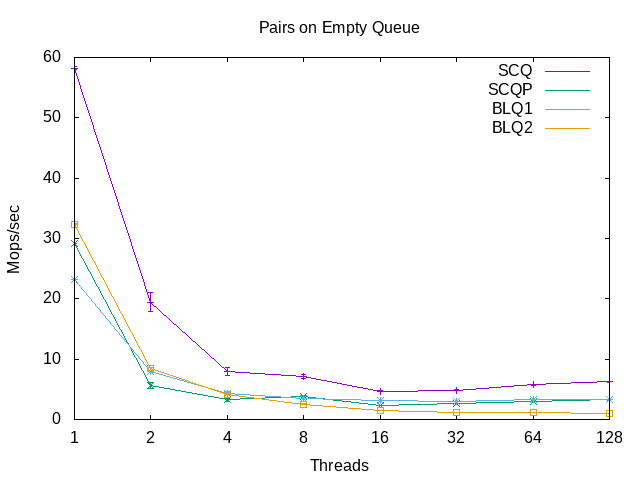
\includegraphics[width=0.49\textwidth]{Pictures/tp_pairs_empty.png}
	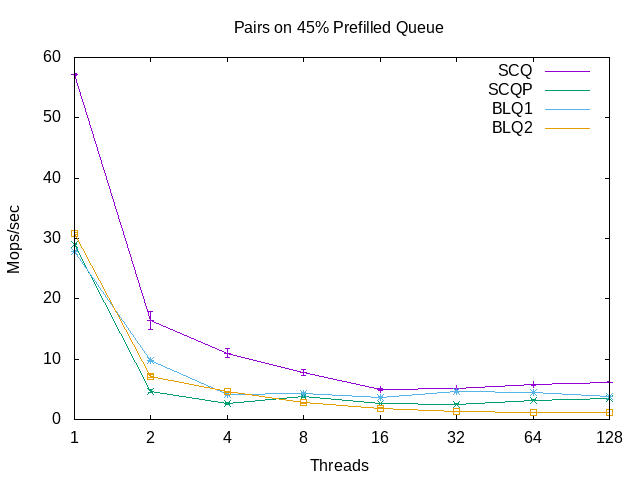
\includegraphics[width=0.49\textwidth]{Pictures/tp_pairs_90.png}
	\caption{Enqueue-dequeue pairs on an empty queue (left) and 45\% prefilled queue (right)}
	\label{fig:tp_pairs}
\end{figure}


Next is the benchmark on enqueue-dequeue pairs, the results can be seen in fig. \ref{fig:tp_pairs}. The results of empty and prefilled queues look very similar, except for SCQ where prefilling seems to make the throughput drop slower with increasing the number of threads.  We can see that SCQ is the clear winner here. It is the fastest for every number of threads and its speed when executed with only one thread is almost twice as fast at the rest. When it comes to comparing the other queues there is no clear cut winner between SCQP, BLQ1 and BLQ2. For a low number of threads BLQ2 is the best while for a higher number of threads SCQP and BLQ1 both perform better. When we compare the results of SCQ with the paper we can see that our benchmarks partly look like the benchmarks on the Intel Xeon CPU and partly like the ones done on the Power PC.
We can see the same strong spike at one thread that can be seen on the Intel Xeon CPU with a very similar throughput ($\approx 60$ Mops/sec) and at two threads drops to a very similar throughput ($\approx 20$ Mops/sec). After four threads we have a drop off that looks similar to what happens on the Power PC. Although, in the paper there was an increase in throughput when going from two to eight threads on the Intel Xeon CPU and when going from one to four threads on PowerPC, we did not observe any such increase.


\begin{figure}[hbtp]
	\centering
	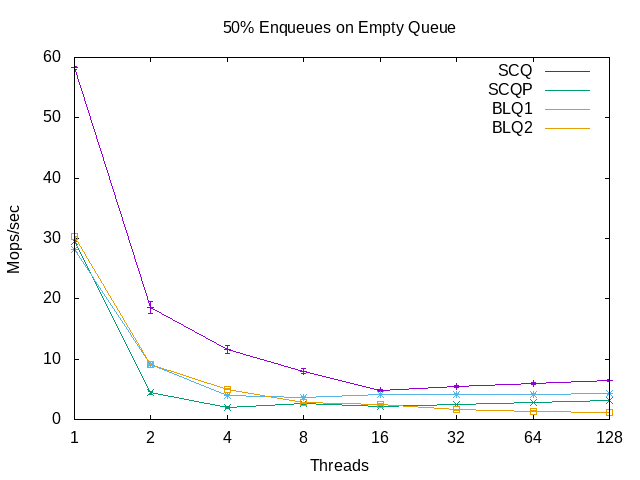
\includegraphics[width=0.49\textwidth]{Pictures/tp_50enq_empty.png}
	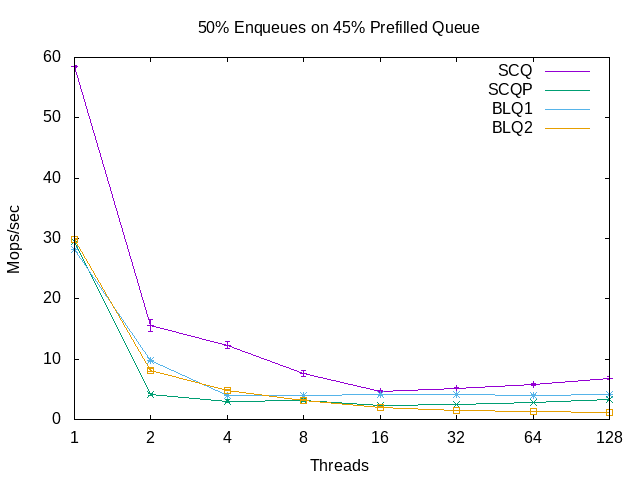
\includegraphics[width=0.49\textwidth]{Pictures/tp_50enq_90.png}
	\caption{Enqueues and dequeues with a 50\% probability each on an empty queue (left) and 45\% prefilled queue (right)}
	\label{fig:tp_enqdeq50}
\end{figure}

The throughput of randomly enqueueing and dequeueing  with a probability of 50\% each can be seen in fig. \ref{fig:tp_enqdeq50}. The results of all queues are very similar to the results of pairwise operations (see fig $\ref{fig:tp_pairs}$). This is interesting because in the paper  pairs performed slightly worse than 50/50 random operations.  Again the behavior of empty or prefilled queues is very similar and SCQ is the clear winner. When it comes to this operation mix it seems like BLQ1 is always preferable over SCQP as it consistently has a higher throughput.

\begin{figure}[hbtp]
	\centering
	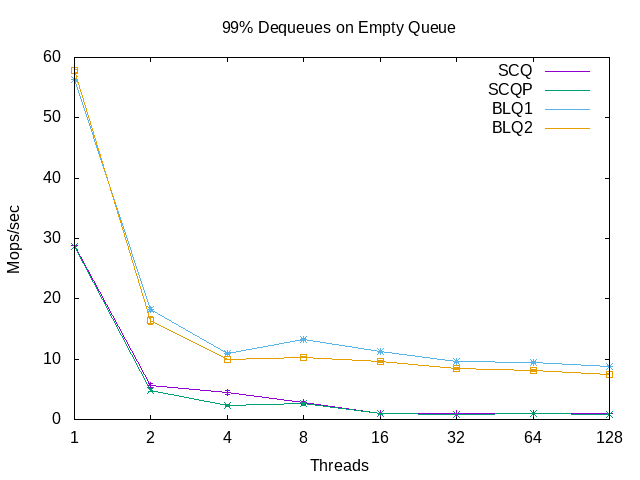
\includegraphics[width=0.75\textwidth]{Pictures/tp_99deq_empty.png}
	\caption{Throughput of 99\% dequeue and 1\% enqueue operations measured on an empty queue}
	\label{fig:tp_99deq}
\end{figure}


We have seen in fig. \ref{fig:tp_empty} that dequeues on an empty SCQ or SCQP are ridiculously fast. This is something that can also be seen in the paper. However, while this is certainly very interesting, it is also slightly misleading. 
The reason why it is so fast is that SCQ can circumvent most of its expensive operations when the $threshold$ is less than zero. However, just because SCQ is empty does not mean that the $threshold$ value is less than zero. This is only the case after initialization or after the queue has failed $3n - 1$ times to find an entry during dequeueing. This means that if we have an empty queue on which we perform dequeues, then a single enqueue operation will make its performance much worse until the $threshold$ value is again less than zero.

To show this we performed a mix of random enqueues and dequeues with a 99\% chance to dequeue. This means that on average the queue will be empty during almost all operations. The results can be seen in fig. \ref{fig:tp_99deq}. This paints a completely different picture: suddenly both SCQ and SCQP are significantly worse than both BLQ1 and BLQ2. Instead of achieving over 3000 Mops/sec the best result for the SCQ is suddenly only 30 Mops/sec. We will investigate the reasons for this in the Section \ref{sec:diss}.

\begin{figure}[H]
	\centering
	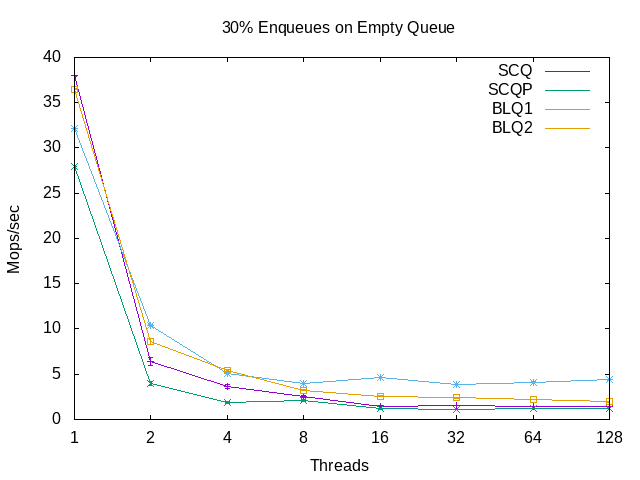
\includegraphics[width=0.49\textwidth]{Pictures/tp_30enq_empty.png}
	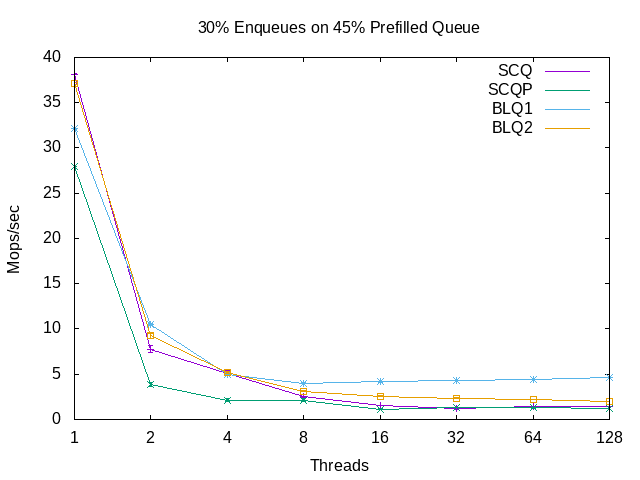
\includegraphics[width=0.49\textwidth]{Pictures/tp_30enq_90.png}
	\caption{Enqueues and dequeues with a 30\% probability to enqueue on an empty queue (left) and 45\% prefilled queue (right)}
	\label{fig:tp_enqdeq30}
\end{figure}

We have already shown that SCQ is generally better than BLQ1 and BLQ2 when the number of enqueues and dequeues are balanced. Balanced means that the number of enqueues and dequeues is approximately the same. Operation mixes for which is this the case are enqueue-dequeue pairs and randomly enqueuing and dequeing with a 50\% probability for each. However, the previous experiment (see fig. \ref{fig:tp_99deq}) shows that this is not necessary the case for unbalanced operation mixes. Since the paper did not test any unbalanced mixes we did tests of enqueues and dequeues with a 30\% chance to enqueue (see fig. \ref{fig:tp_enqdeq30}). For one thread SCQ and BLQ2 perform very similarly, but already here we can see that SCQ only achieves $\approx 38$ Mops/sec compared to the $\approx 60$ Mops/sec it had under the more balanced loads (see fig. \ref{fig:tp_enqdeq50} and \ref{fig:tp_pairs}). At a higher number of threads we can clearly see that both BLQ1 and BLQ2 are superior to SCQ and SCQP, with BLQ1 being the winner. In these experiments SCQP had the worst performance. This shows that the more sophisticated SCQ and SCQP are not necessarily better than the simpler BLQ1 and BLQ2.

Let us now revisit our initial hypotheses from Section~\ref{sec:initial_theories}. The first hypothesis was that the throughput of BLQ1 and BLQ2 will not scale with the number of threads. All of our experiments support this hypothesis. The second hypothesis was that when it comes to dequeues on an empty queue, both SCQ and SCQP should have a very high throughput that scales with the number of threads. This has only been partially true: the throughput of SCQ and SCQP is remarkably high but it seems to only scale for up to 4 threads, afterwards the throughput slowly decreases (see fig. \ref{fig:tp_empty}). The final hypothesis was that we expected SCQP to perform worse than SCQ. This has held true, we have seen cases in which they have very similar performance (for example fig. \ref{fig:tp_empty} or \ref{fig:tp_99deq}) but we have not seen a case where SCQP outperforms SCQ. This is in contrast to the paper where SCQP in rare occasions outperforms SCQ.


\subsubsection{Benchmarking an Optimization to SCQ}
\label{sec:bench_opt}

One of the optimizations for SCQ is to let a dequeuer spin for a short amount of time if it arrives at an entry before an enqueuer can store a value there. By spinning we mean that the thread loops through a simple operation $k$ times. Since \cite{nikolaev2019scalable} did not provide any instructions on how to choose $k$, it was chosen on the basis of a series of benchmarks (see fig. \ref{fig:wait}). This optimization does not seem to have a big impact. As we can see there is no clear best $k$, so we decided to use $k=1000$ as this had the best performance for randomly enqueuing and dequeing with a 50\% probability for each.

\begin{figure}[H]
	\centering
	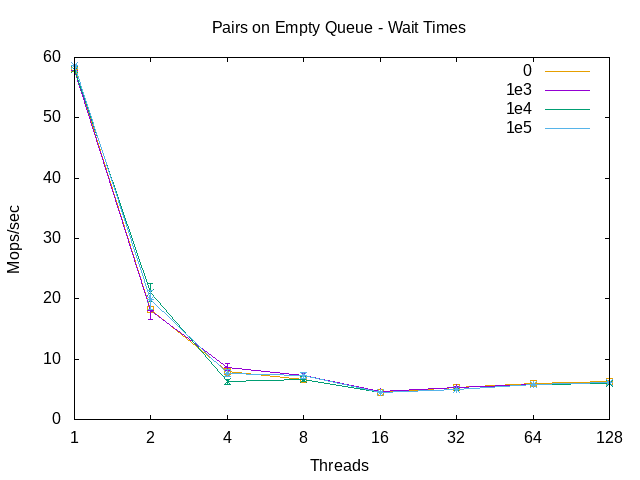
\includegraphics[width=0.49\textwidth]{Pictures/wait_pairs.png}
	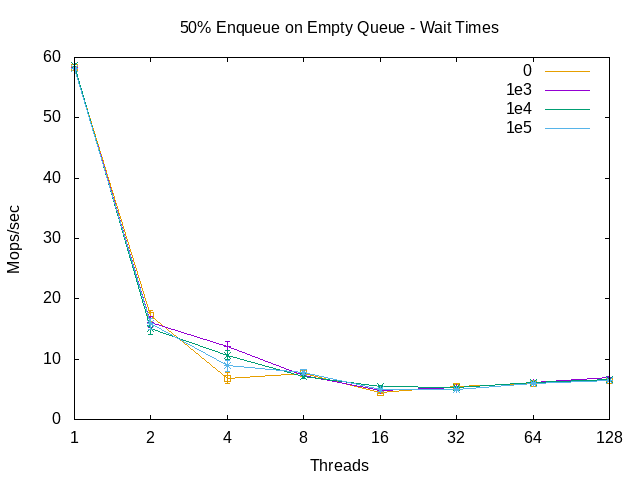
\includegraphics[width=0.49\textwidth]{Pictures/wait_enqdeq50.png}
	\caption{Throughput of different number of loops for enqueue-dequeue pairs (left) and enqueues and dequeues with a 50\% probability each (right) on an empty queue}
	\label{fig:wait}
\end{figure}


\subsection{Benchmarking  the Inner Workings of SCQ}
\label{sec:diss}
We have already shown that the throughput of SCQ heavily depends on the mix of operations. Now we want to investigate why this is the case. Since SCQP consists only of two SCQs we decided to focus on SCQ. To do this we change the SCQ class to benchmark certain internal characteristics. We count:
\begin{samepage}
\begin{itemize}
	\item \textbf{Enqueue:} 
	\begin{itemize}
		\item How often \textit{enqueue} needs to loop to successfully enqueue a value
		\item How often the CAS writing a new entry fails
		\item How often we try to access an unsafe entry
	\end{itemize}
	\item \textbf{Dequeue:}
	\begin{itemize}
		\item How often \textit{dequeue} needs to loop to successfully dequeue a value 
		\item How often \textit{dequeue} tries to access an old entry ($cycle(entry)<cycle(head)$)
		\item How often the CAS that changes the old element fails
		\item How often we call \textit{catchup}
	\end{itemize}
\end{itemize}
\end{samepage}
	
We normalize all of these counts by how often the corresponding operation happens, for example if we have 200 CAS fails in 400 enqueue operations then we report a relative count of 0.5. Then we rerun all the experiments from section~\ref{sec:bench} with this new setup. We report mean values and standard deviations.
%Some simple sanity checks are: there should be no CAS fails for one thread and the number of CAS fails in \textit{dequeue} should be smaller than the number of accesses to an old entry in \textit{dequeue} (this is because the dequeuer only uses CAS on write on old entries). 

Since under these metrics unbalanced operations mixes perform significantly worse than balanced mixes we first show the graphs with all of the operation mixes and afterwards with only the balanced ones.  Note that some operation mixes do not appear in some graphs, this is because this operation mix did not do the required operation (it makes no sense the include an experiment with only dequeues in the graph about enqueue CAS fails).

\subsubsection{Unbalanced Operations}

\begin{figure}[H]
	\centering
	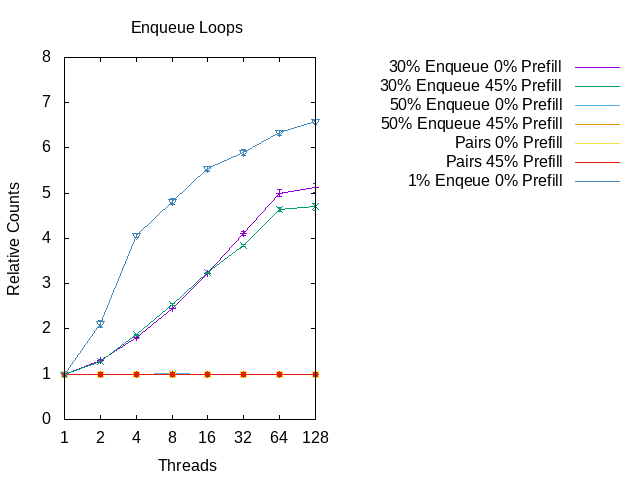
\includegraphics[width=0.49\textwidth]{Pictures/diss_enq_loops.png}
	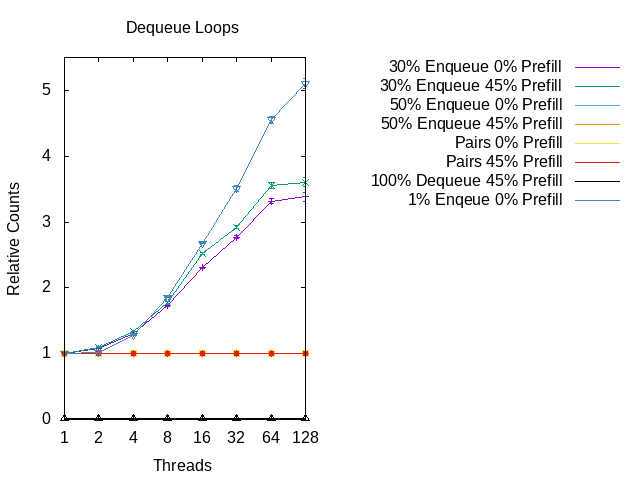
\includegraphics[width=0.49\textwidth]{Pictures/diss_deq_loops.png}
	\caption{Relative number of loops, left: enqueue loops; right: dequeue loops}
	\label{fig:diss_loops}
\end{figure}

\begin{figure}[H]
	
	\centering
	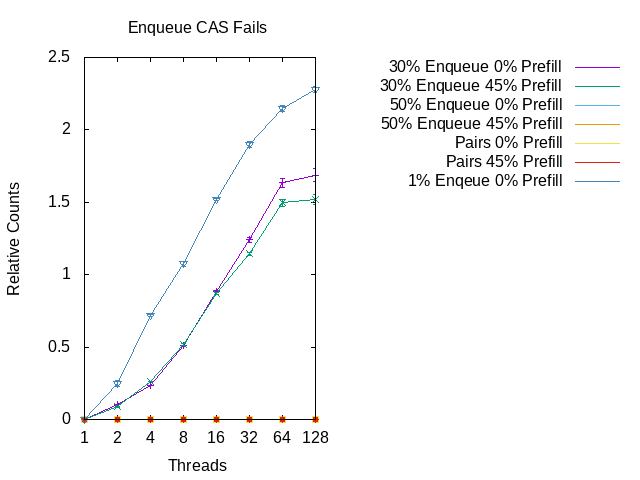
\includegraphics[width=0.49\textwidth]{Pictures/diss_enq_cas.png}
	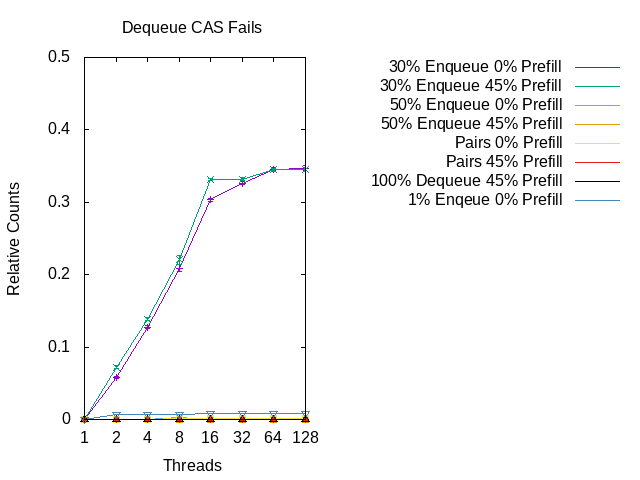
\includegraphics[width=0.49\textwidth]{Pictures/diss_deq_cas.png}
	\caption{Number of CAS fails per operation, left: enqueue CAS fails; right: dequeue CAS fails}
	\label{fig:diss_cas_fails}
\end{figure}

\begin{figure}[H]
	\centering
	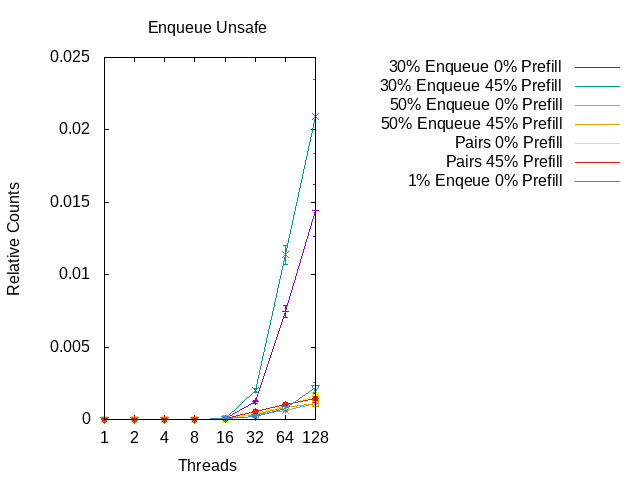
\includegraphics[width=0.7\textwidth]{Pictures/diss_enq_unsafe.png}
	\caption{Average number of times enqueue accesses an unsafe entry}
	\label{fig:diss_enq_unsafe}
\end{figure}

\begin{figure}[H]
	\centering
	
	\minipage{0.49\textwidth}
	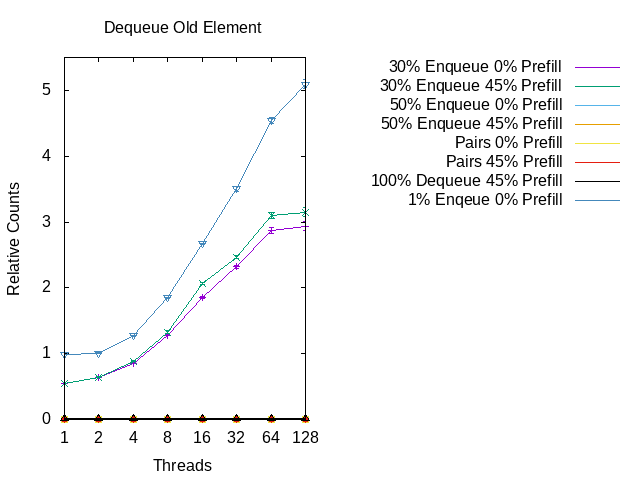
\includegraphics[width=\textwidth]{Pictures/diss_deq_old.png}
	\caption{Average number of times dequeue tried to access an old element}
	\label{fig:diss_deq_old}
	\endminipage\hfill
	\minipage{0.49\textwidth}
	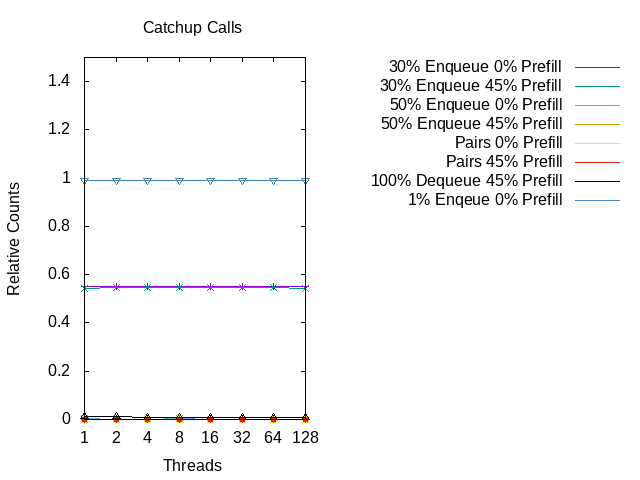
\includegraphics[width=\textwidth]{Pictures/diss_deq_catchup.png}
	\caption{Average number of catchup calls per dequeue}
	\label{fig:diss_catchup}
	\endminipage\hfill
\end{figure}

The results of these experiments can be found in fig. \ref{fig:diss_loops}, \ref{fig:diss_cas_fails}, \ref{fig:diss_enq_unsafe},  \ref{fig:diss_deq_old} and \ref{fig:diss_catchup}.
As we can see unbalanced distributions (1\% enqueue/99\% dequeue and 30\% enqueue/70\% dequeue) perform way worse in all of the measurements than balanced distributions. Balanced distributions need on average one loop per enqueue / dequeue operation, unbalanced distributions need several more and the number of loops they need scales with the number of threads (fig. \ref{fig:diss_loops}). Unbalanced distributions have a very high number of CAS fails (fig. \ref{fig:diss_cas_fails}) that even scales with the number of threads. Furthermore, their dequeue operation tries to dequeue an old element significantly more often and they have the highest amount of catchup calls. A general trend for these unbalanced operation mixes is that the experiments with 30\% enqueue/70\% dequeue on empty or prefilled queues perform about the same and the experiment with 1\% enqueue/99\% dequeue  is significantly worse. So even for unbalanced distributions it seems to hold that more unbalanced distributions are worse than less unbalanced distributions.

The primary reason why unbalanced distributions have such a bad throughput should be the high number of CAS fails, as these are very expensive when it comes to computation time. A CAS fail can only happen if a dequeuer arrives at an entry before an enqueuer has written to it.\footnote{Or when two enqueuers from different cycles are at the same entry, which can only happen if a thread sleeps for an entirely cycle which is very unlikely.} This is only likely to happen if the head overtakes the tail which happens when we dequeue more values than we enqueue. This also explains the high number of \textit{catchup} calls (see fig. \ref{fig:diss_catchup}) for unbalanced operations: $catchup$ is used to put the tail in front of the head, so it only gets called when the head overtakes the tail.


%Let us first consider the number of loops an enqueue or dequeue takes (fig. \ref{fig:diss_loops}). Most mixes of operations take on average one loop. An exception to this are dequeues on a prefilled queue and dequeues on an empty queue\footnote{Only dequeues on an empty queue is not show in any graph as all the measured counts were 0.} both of which take on average 0 loops. This makes sense because after a small number of dequeues both queues are definitely empty and have $threshold=-1$ at which point they only need to do a $threshold$ lookup to complete. Another exception are unbalanced operation mixes: both 1\% enqueue/ 99\% dequeue and 30 \% enqueue/ 70\% dequeue take considerably more than one loop to complete their operations. Furthermore, their number of loops increases with the number of threads. This is the first cause why unbalanced operation mixes had a way worse throughput than more balanced ones. 

%Now we will analyze the number of CAS fails (see fig. \ref{fig:diss_cas_fails}), since CAS fails are expensive a good datastructure should try and avoid having many of them. Most of the operation mixes have a negligible amount of CAS fails with three exceptions: 1\% enqueue/ 99\% dequeue and 30 \% enqueue/ 70\% dequeue operation mixes have a significant amount of CAS fails. What is even worse is that the number of enqueue CAS fails increases linearly for them. At 32 threads all of the three have on average at least one CAS fail per enqueue operation which seems to us like it is a lot. This ridiculous number of CAS fails explains why the SCQ is worse than the BLQ1 and BLQ2 for unbalanced operation mixes.

\subsubsection{Balanced Operations}

\begin{figure}[H]
	\centering
	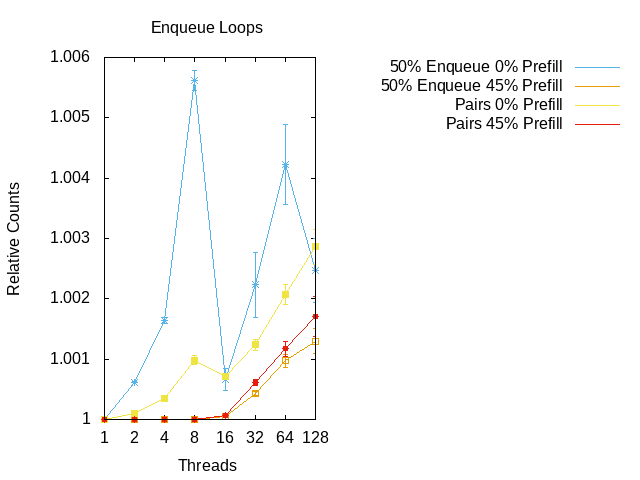
\includegraphics[width=0.49\textwidth]{Pictures/diss_enq_loops_red.png}
	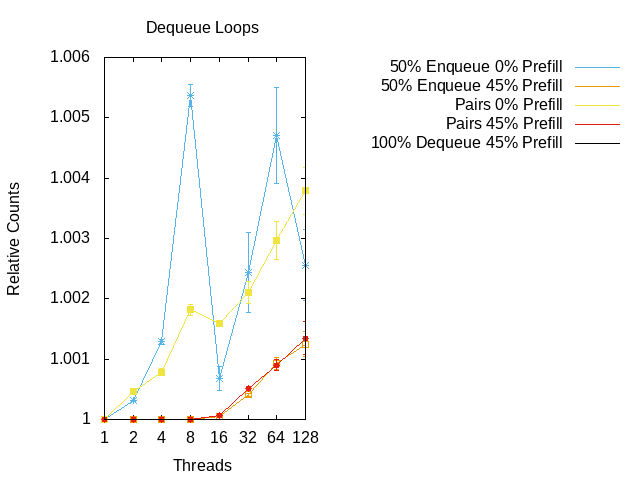
\includegraphics[width=0.49\textwidth]{Pictures/diss_deq_loops_red.png}
	\caption{Relative number of loops, left: enqueue loops; right: dequeue loops}
	\label{fig:diss_red_loops}
\end{figure}

\begin{figure}[H]
	\centering
	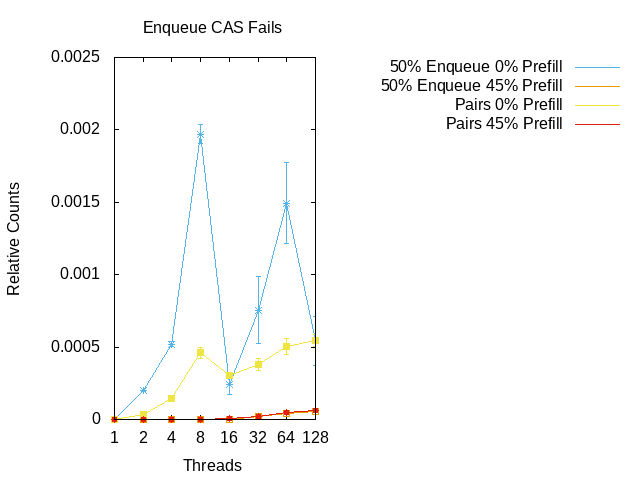
\includegraphics[width=0.49\textwidth]{Pictures/diss_enq_cas_red.png}
	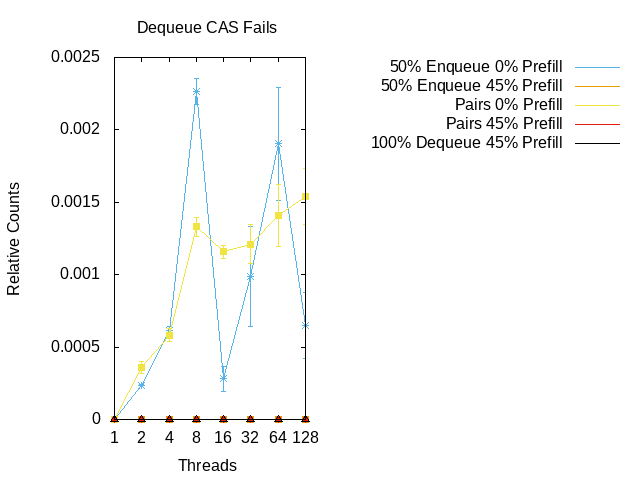
\includegraphics[width=0.49\textwidth]{Pictures/diss_deq_cas_red.png}
	\caption{Number of CAS fails per operation, left: enqueue CAS fails; right: dequeue CAS fails}
	\label{fig:diss_red_cas_fails}
\end{figure}

\begin{figure}[H]
	\centering
	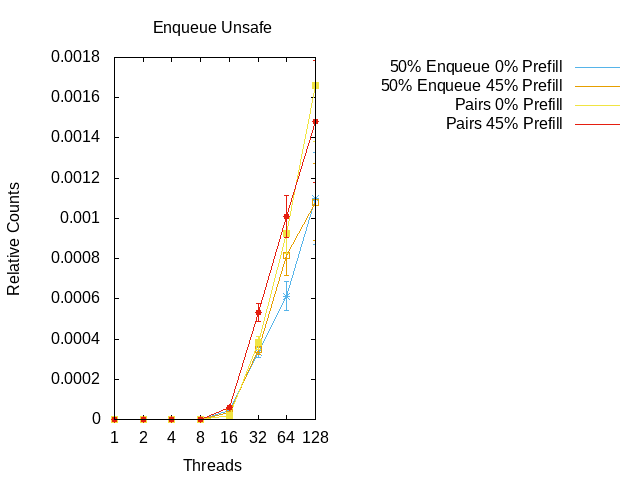
\includegraphics[width=0.7\textwidth]{Pictures/diss_enq_unsafe_red.png}
	\caption{Average number of times enqueue accessed an unsafe entry}
	\label{fig:diss_red_enq_unsafe}
\end{figure}

\begin{figure}[H]
	\centering
	
	\minipage{0.49\textwidth}
	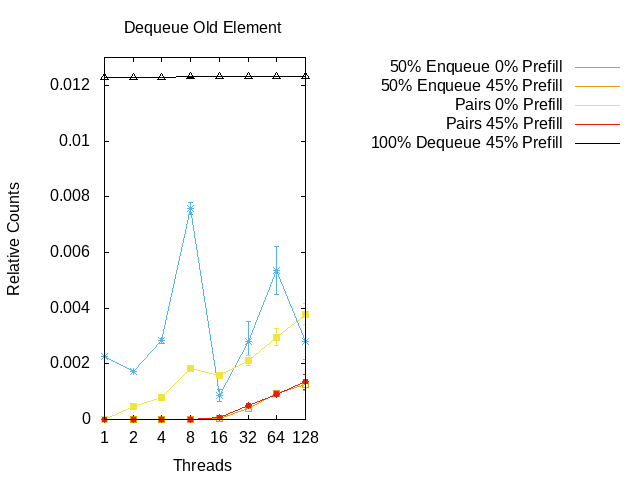
\includegraphics[width=\textwidth]{Pictures/diss_deq_old_red.png}
	\caption{Average number of times dequeue tried to access an old element}
	\label{fig:diss_red_deq_old}
	\endminipage\hfill
	\minipage{0.49\textwidth}
	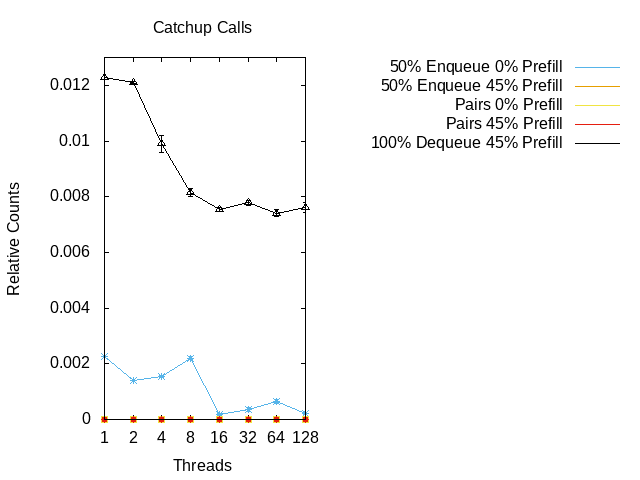
\includegraphics[width=\textwidth]{Pictures/diss_deq_catchup_red.png}
	\caption{Average number of catchup calls per dequeue}
	\label{fig:diss_red_catchup}
	\endminipage\hfill
\end{figure}

We present the benchmarks for the balanced distributions in fig.\ \ref{fig:diss_red_loops}, \ref{fig:diss_red_cas_fails}, \ref{fig:diss_red_enq_unsafe}, \ref{fig:diss_red_deq_old} and \ref{fig:diss_red_catchup}. When considering the loops per operation it is very obvious that there is an increase when going over 16 threads (see fig. \ref{fig:diss_red_loops}). A similar increase can be observed for enqueue CAS fails (fig. \ref{fig:diss_red_cas_fails} left), unsafe enqueues (fig. \ref{fig:diss_red_enq_unsafe}) and dequeues of old elements (fig. \ref{fig:diss_red_deq_old}). We cannot find a good reason for why this increase happens, but we think that this might have something to do with the CPU, since this behavior is consistent for all the balanced operation mixes.
%This is interesting as 16 is also the number of cores per CPU that Nebula has, meaning for a higher number of threads we need to distribute work between different CPUs. This could potentially lead to situations where an enqueuer takes longer to enqueue a value meaning that a dequeuer has more time to arrive there and change the value (which can cause a CAS fail in the enqueuer or the dequeuer). The authors of the paper noticed a significant drop in throughput after they went over they had more threads than the number of CPUs per core. 

As you might have noticed, enqueues on an empty queue are completely missing from all of the presented benchmarks. The reason for this is that in this case all performance counters are 0 or NaNs. This implies that SCQ works correctly: when dequeuing on an empty SCQ the $threshold$ optimization allows us to bypass all the expensive procedures measured by the performance counters. Unfortunately, this does not explain why the throughput decreases when using more than 4 threads.


Something that these benchmarks fail to show is the reason why  pairwise operations perform very similarly to balanced random mixes, unlike the paper where pairs perform a bit worse.  Pairwise operations have a very low number of loops and CAS fails up to 16 threads. Intuitively this would mean that they are way faster than random balanced operation mixes as these have more loops/fails. We think that the primary reason why this has so little influence is that the scale of these plots is rather small. For example the highest relative count of enqueue CAS fails is about $0.002$ which is equivalent to one CAS fail every 500 enqueue operation. This seems like a rather small amount of CAS fails, which explains why the different balanced operation mixes show only small differences in performance.

Another thing that we cannot explain with these benchmarks is the reason why the throughput in section~\ref{sec:bench} is different from the throughput reported in \cite{nikolaev2019scalable}. In my opinion, none of the measured performance counters seem atypical or can explain the difference. Thus we believe that the biggest reason for the discrepancies is the fact that we benchmarked on different systems and that Nikolaev is a more experienced developer who implemented SCQ in a more efficient way.

Finally, fig. \ref{fig:diss_red_catchup} shows that \textit{catchup} calls are only likely for queues with random operation mixes that are not prefilled. It makes sense that pairwise operation mixes have no \textit{catchup} calls because all of the pairs used enqueue before the dequeue. This means that the head can never get in front of the tail, which means no catchup calls. A catchup call is also much less likely if the queue is prefilled, because this means that initially the tail pointer is a number of entries ahead of the tail pointer (this is the number of prefilled elements) which makes it much less likely for the head to overtake the tail.


%We first take a look at pairwise operations, the graphs show that they have a very low number of enqueue/dequeue loops, enqueue/dequeue CAS fails, unsafe enqueues and dequeues of old elements. However all of this metrics start drastically increasing after 16 threads. This is interesting as 16 is also the number of cores per CPU that Nebula has, meaning for a higher number of threads we need to distribute work between different CPUs. This could potentially lead to situations where enqueuer take longer to enqueue a value meaning that a dequeuer has more time to arrive there and change the value (which can cause a CAS fail in the enqueuer or the dequeuer). The authors of the paper noticed a significant drop in throughput after they went over they had more threads than the number of CPUs per core. This could partly explain it.

\section{Conclusion}
In this project, we implemented SCQ, SCQP, BLQ1 and BLQ2 and recreated most of the experiments in the paper. Our SCQ shows a very similar behavior at a lower number of threads to SCQ from the paper. At a higher number of threads our SCQ performs worse, which we think is due to different computers and Nikolaev being the more experienced developer. Our experiments showed that SCQ is superior to SCQP, BLQ1 and BLQ2 when it comes to balanced operation mixes and dequeues on an empty queue.

We leveraged our theoretical understanding of SCQ to construct experiments in which it performed dramatically worse. If the operation mix is skewed so that it consists of more dequeues than enqueues then the behavior of SCQ and SCQP becomes drastically worse than BLQ1 and BLQ2. This goes to show that the more advanced lock-free queue is not always better than a simpler queue with locks. In the end one needs to consider what kind of operation mixes they need.


\pagebreak


\bibliographystyle{acm}
\bibliography{verzeichnis}

\section*{Internet Sources}
I did my best to collect all the internet sources I used.
\begin{itemize}
	\item \url{https://stackoverflow.com/questions/38999911/what-is-the-best-way-to-realize-a-synchronization-barrier-between-threads} I used ``UmNyobe'''s barrier implementation and changed it so that it keeps the time of when the threads are allowed to pass through.
	\item \url{https://stackoverflow.com/} I asked for help with my implementation of a benchmark, turns out I was measuring the inverse latency instead of the throughput.
	\item \url{https://www.uni-muenster.de/AMM/num/Vorlesungen/WissenschaftlichesRechnen_WS1516/Material/multithreading.pdf} For the basics of how to use C++ threads.
	\item 
	\url{https://en.wikipedia.org/wiki/Linear_congruential_generator} In the lecture we heard that some of the RNG are not threadsafe, since I had troubles finding out which RNGs are threadsafe I made my own which is a linear congruential generator. I selected parameters from \cite{LinCongrGen}.
\end{itemize}

\end{document}
